\newpage
\section{Quantum Entanglement}


\subsection{Multiple Qubits and Tensor Products}

\subsubsection{Tensor Products}
A pair of classical bits can have (or be in) any of the four possible states $00, 01, 10, 11$. 

If a bit is represented by $\ket{0}=\begin{pmatrix}
    1 \\0
\end{pmatrix}$ and $\ket{1}=\begin{pmatrix}
    0\\1
\end{pmatrix}$, the two-bit states can be represented by four column vectors
\begin{align*}
    \ket{00}=\begin{pmatrix}
        1\\0\\0\\0
    \end{pmatrix},\ 
    \ket{01}=\begin{pmatrix}
        0\\1\\0\\0
    \end{pmatrix}, \ 
    \ket{10}=\begin{pmatrix}
        0\\0\\1\\0
    \end{pmatrix},\ 
    \ket{11}=\begin{pmatrix}
        0\\0\\0\\1 
    \end{pmatrix},
\end{align*}
They are examples of tensor products. 

In general, the \hl{tensor product} of an $m\times n$ matrix (vector) $A$ and a $p \times q$ matrix (vector) $B$ is an $mp \times nq$matrix in the form
\begin{align*}
    A\otimes B=\begin{pmatrix}
        a_{11}B & \cdots & a_{1n}B\\
        \vdots & \ddots & \vdots\\
        a_{m1}B & \cdots & a_{mn}B
    \end{pmatrix}
\end{align*}
The tensor product of two vectors $\ket{u}$ and $\ket{v}$ is often abbreviated as $\ket{u}\ket{v}$ or $\ket{uv}$, as was done above.

\begin{align*}
    \sigma_{1x}=\sigma_x \otimes I, \ \sigma_{1y}=\sigma_y \otimes I,\ \sigma_{1z}=\sigma_z \otimes I\\
    \sigma_{2x}=I \otimes \sigma_x, \ \sigma_{2y}=I \otimes \sigma_y,\ \sigma_{2z}=I \otimes \sigma_z
\end{align*}

\subsection{Entangled States and EPR Paradox}

\subsubsection{Combining Two Qubits}
In the case of two qubits the vector space is, therefore, four-dimensional, with an orthonormal basis
\begin{align*}
    \ket{00},\ \ket{01},\ \ket{10},\ \ket{11}
\end{align*}

The general state $\ket{\Psi}$ that nature allows us to associate with two qubits is any normalized superposition of the four orthogonal classical states,
\begin{align*}
    \ket{\Psi}=\alpha_1\ket{00}+\alpha_2\ket{01}+\alpha_3\ket{10}+\alpha_4\ket{11}
\end{align*}
with the complex amplitudes being constrained only by the normalization condition $1$. 

In other words, two-qubit states are unit vectors in $\left(\mathbb{C}^2\right)^{\otimes 2}=\mathbb{C}^2\otimes \mathbb{C}^2$. 
\begin{itemize}
    \item If the first qubit is in $\alpha_1\ket{0}+\beta_1\ket{1}$, and the second qubit is in $\alpha_2\ket{0}+\beta_2\ket{1}$, then the \hl{product state} is
    \begin{align*}
        &(\alpha_1\ket{0}+\beta_1\ket{1}) \otimes (\alpha_2\ket{0}+\beta_2\ket{1})\\
        =\ &\alpha_1\alpha_2\ket{00}+\alpha_1\beta_2\ket{01}+\beta_1\alpha_2\ket{10}+\beta_1\beta_2\ket{11}
    \end{align*}
    \item In the two case, even though we put the two qubits together, the information they encode is still separable. If we operate on the first qubit only, the second remains unchanged:
    \begin{align*}
        (L\otimes I)(\ket{u} \otimes \ket{v})=(L\ket{u})\otimes \ket{v}
    \end{align*}
\end{itemize}

It takes 4 real parameters to specify a two-qubit product state (or separable state). But, it takes 6 real parameters to specify the most general two-qubit state.

Obviously, the space of all two-qubit states is much richer than that of the product states, which can be prepared separately for each qubit.

The other class of states are known as the \hl{entangled states}, exemplified by the famous Bell states. One of the four Bell states is
\begin{align*}
    \ket{\Psi_+}=\frac{1}{\sqrt{2}}(\ket{01}+\ket{10})
\end{align*}
In the state particle 1 can be in state $\ket{0}$ and particle 2 in state $\ket{1}$, or vice versa, but there is no way of knowing which particle is in which state. All that is defined is the fact that the two qubits are different.

\subsubsection{EPR Paradox}
Entanglement is closely linked to the issue of locality (or non-locality) in quantum theory. In particular, if the two particles in an entangled state are widely separated, then a measurement on one will immediately influence the quantum state of the other one. It seems as if the particles are communicating faster than the speed of light.

In Bohm’s version of the EPR paradox, the two particles are in the Bell state
\begin{align*}
    \ket{\Psi_+}=\frac{1}{\sqrt{2}}(\ket{01}+\ket{10})
\end{align*}
One can measure the first qubit according to the following measurement rule
\begin{figure}[H]
    \centering
    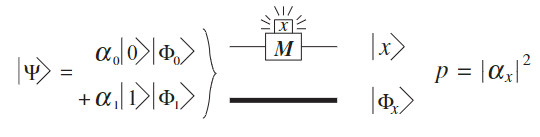
\includegraphics[width=0.309\textwidth]{QI4/EPR}
\end{figure}

Upon the measurement of particle 1, one knows the state of the faraway particle 2 instantaneously. Indeed, modern experiments have confirmed that their properties remain entangled after they are sent far apart.

However, the special theory of relativity is not violated because no information travels faster than light (local in the quantum field theoretical sense). Before the measurement, particle 2 has equal probabilities in states $\ket{0}$ and $\ket{1}$. This remains to be true (in terms of an external observer’s statistical model) after the measurement. The measurement of particle 1 does not a priori fix the state of particle 2; there is no information transfer. (其实信息传递并无超光速, 即纠缠虽然状态相反, 但并未传递信息, 信息是在之前就已传到了)

\subsubsection{Information in the Bell State}
The two-particle Bell state cannot be written as the tensor product of single-particle states. The single-particle states are entangled, not separable, in such superpositions. This means that all of the information is distributed among two qubits (i.e., not local), and that none of the individual systems carries any information. This is the essence of entanglement and is one of the novel and counterintuitive features of quantum mechanics. For further illustration, we introduce the concept of expectation values, or average values.

Suppose we consider an experiment that measures an observable $L$, whose eigenvalues are $\lambda$ with corresponding eigenvectors $\ket{\lambda}$, i.e., $L\lambda=\lambda\ket{\lambda}$. 

Suppose that the normalized state of a quantum system is $\psi$, which can be expanded in the orthonormal basis $\left\{ \ket{\lambda} \right\}$: 
\begin{align*}
    \ket{\psi}=\sum_{\lambda}\ket{\lambda}\braket{\lambda|\psi}
\end{align*}

Let $L$ operate on $\psi$: 
\begin{align*}
    L\ket{\psi}=\sum_{\lambda}L\ket{\lambda}\braket{\lambda|\psi}=\sum_{\lambda}\lambda\ket{\lambda}\braket{\lambda|\psi}
\end{align*}

The \hl{expectation value (期待值)} of $L$ of the system is defined as
\begin{align*}
    \braket{L}\equiv \braket{\psi|L|\psi}=\sum_{\lambda}\lambda\braket{\psi|\lambda}\braket{\lambda|\psi}=\sum_{\lambda}\lambda P(\lambda)
\end{align*}
This is the weighted sum of $L$'s eigenvalues $\lambda$ with probability $P(\lambda)=\braket{\psi|\lambda}\braket{\lambda|\psi}$. 

Suppose we perform a large number of identical experiments. We can identify $P(\lambda)$ as the percentage of observations whose result is $\lambda$. In the statistical sense, the experimental average is identical to the mathematical definition of $\braket{L}$.

For a one-qubit state $\ket{\psi}=\cos\frac{\theta}{2}\ket{0}+e^{i\phi}\sin\frac{\theta}{2}\ket{1}$ one can always find a particular direction $\hat{n}$ for which $\braket{\vec{\sigma}\cdot\hat{n}}=1$. One can check $\hat{n}=(\sin\theta\cos\phi,\ \sin\theta\sin\phi,\ \cos\theta) $ is the direction. This still holds when we measure one of the qubit in a two-qubit product state, such as $\ket{\psi}\otimes\ket{\psi'}$.

However, if one measures the first qubit in the Bell state $\ket{\Psi_+}$, the result is $\braket{\vec{\sigma}^{(1)}\cdot\hat{n}}=0$ for any $\hat{n}$. Let us operate $\sigma_n^{(1)}=\vec{\sigma}^{(1)}\cdot\hat{n}$, or more precisely $1$: 
\begin{align*}
    \sigma_n^{(1)}\ket{\Psi_+} \propto\ & (\cos\theta\ket{0}+e^{i\phi}\sin\theta\ket{1})\ket{1}\\
    +&(e^{-i\phi}\sin\theta\ket{0}-\cos\theta\ket{1})\ket{0}
\end{align*}
A quick comparison with $\ket{\Psi_+}\propto  \ket{01}+\ket{01}$ shows that
\begin{align*}
    \braket{\Psi_+| \vec{\sigma}^{(1)}\cdot\hat{n} |\Psi_+}=0
\end{align*}
regardless of the direction of $\hat{n}$. 

If the expectation value of a component of $\vec{\sigma}^{(1)}$ vanishes, it means that the experimental outcome is equally likely to be $\pm 1$. In other words, the outcome is completely uncertain. Assume Charlie prepare two qubits in the entangled state and send one qubit to Alice and one to Bob without looking at (i.e., measuring) the qubits. Although Alice and Bob know exactly what the combined system is in, they can predict nothing about the outcome of their individual measurements. 

We have constructed the dot product of the vector-operator $\vec{\sigma}^{(1)}$ and $\vec{\sigma}^{(2)}$, which is manifestly rotational invariant,
\begin{align*}
    \vec{\sigma}^{(1)}\cdot\vec{\sigma}^{(2)}=\sigma_x^{(1)}\sigma_x^{(2)}+\sigma_y^{(1)}\sigma_y^{(2)}+\sigma_z^{(1)}\sigma_z^{(2)}
\end{align*}
This operator always yields a certain information:
\begin{align*}
    \braket{\Psi_+| \vec{\sigma}^{(1)}\cdot\vec{\sigma}^{(2)} |\Psi_+}=const
\end{align*}

\subsection{Density Matrices}
A complete description of the Bell state involves the variables both at Alice and Bob’s ends. To evaluate the result of a measurement to be carried out only at, say, Alice’s end, we still operate on the whole state, which involves both ends. To capture the complete information Alice (not Bob) has, we need to introduce new tools: density matrix and reduced density matrix.

We begin our introduction to density matrix with an alternative expression for evaluating the expectation value. First, let us define the \hl{trace (迹)} of an operator $L$ to be
\begin{align*}
    \mathrm{Tr}L=\sum_i \braket{i|L|i}
\end{align*}
where $\left\{ \ket{i} \right\}$ is a complete set of basis vectors. 
\begin{itemize}
    \item The trace of a projection operator is 1. 
    \item The trace of a Hermitian operator is the sum of its eigenvalues. 
\end{itemize}

Recall the completeness condition $\displaystyle \sum_i \ket{i}\bra{i}=I$. 
\begin{align*}
    L=LI=\sum_i L\ket{i}\bra{i}
\end{align*}

The expectation value of $L$ in state $\ket{\psi}$ can be, alternatively, written as 
\begin{align*}
    \braket{\psi|L|\psi}=\sum_i \braket{\psi|L|i}\braket{i|\psi}=\sum_i \braket{i|\psi}\braket{\psi|L|i}
\end{align*}
where we simply reverse the order of the two numbers in the second equality.

According to the definition $ \mathrm{Tr}L=\sum\limits_i \braket{i|L|i}$, 
\begin{align*}
    \braket{\psi|L|\psi}=\mathrm{Tr}\ket{\psi}\bra{\psi}L\equiv\mathrm{Tr} \rho L
\end{align*}
$\rho\equiv \ket{\psi}\bra{\psi}$ is the \hl{density matrix} of the pure state $\ket{\psi}$. 

Density matrix can also be used to described a state of incomplete information. 

For example, Charlie has prepared a qubit and sends it to Alice. He does not tell her along which axis the qubit was prepared. Instead, he tells her that the state is equally likely to be $\ket{0}$ along the $z$ axis or $\ket{r}$ along the x axis. Alice can reason that the expectation value of $L$ is
\begin{align*}
    \braket{L}=\frac{1}{2}\braket{0|L|0}+\frac{1}{2}\braket{r|L|r}=\frac{1}{2}\mathrm{Tr}\ket{0}\bra{0}L + \frac{1}{2}\mathrm{Tr}\ket{r}\bra{r}L
\end{align*}

Now we can define a density matrix $\rho$ that encodes Alice’s knowledge such that $\braket{L}=\mathrm{Tr}\rho L$. 
One can read that the density matrix $\rho$ is half the projection operator onto $\ket{0}$ plus half the projection operator onto $\ket{r}$
\begin{align*}
    \rho=\frac{1}{2}\ket{0}\bra{0}+\frac{1}{2}\ket{r}\bra{r}
\end{align*}
which represents a \hl{mixed state}.

One can generalize $\rho=\sum\limits_i P_i\ket{\psi_i}\bra{\psi_i}$ to be a mixture of projection operators with probabilities $P_i$. 

\subsection{Reduced Density Matrix and Entanglement Entropy}

\subsubsection{Reduced Density Matrix}
Now, for a separable state $\ket{\psi}=\ket{\lambda}_A\ket{\phi}_B$ , the density matrix is
\begin{align*}
    \rho=\ket{\psi}\bra{\psi}=\ket{\lambda}\bra{\lambda}\otimes \ket{\phi}\bra{\phi}=\rho_A \otimes \rho_B
\end{align*}
where we can define \hl{reduced density matrices}
\begin{align*}
    \rho_A=\ket{\lambda}\bra{\lambda},\ \rho_B=\ket{\phi}\bra{\phi}
\end{align*}
as the density matrices separately for each subsystem. Notice that $\rho_A^2=\rho_A$ and , hence, $\mathrm{Tr}\rho_A^2=1$. 

For an entangled state, it is possible to write (known as the \hl{Schmidt decomposition})
\begin{align*}
    \ket{\psi}=\sum_i c_i\ket{\lambda_i}_A\ket{\phi_i}_B
\end{align*}
where $\left\{ \ket{\lambda_i}_A \right\}$ and $\left\{ \ket{\phi_i}_B \right\}$ orthonormal basis sets for the $A$ and $B$ subsystems, respectively. The reduced density matrices are defined as 
\begin{align*}
    \rho_A&=\mathrm{Tr}_B\ket{\psi}\bra{\psi}=\sum_i|c_i|^2\ket{\lambda_i}\bra{\lambda_i}\\
    \rho_B&=\mathrm{Tr}_A\ket{\psi}\bra{\psi}=\sum_i|c_i|^2\ket{\phi_i}\bra{\phi_i}
\end{align*}

In fact, the orthonormal sets $\left\{ \ket{\lambda_i}_A \right\}$ and $\left\{ \ket{\phi_i}_B \right\}$ are the eigenstates of the reduced density matrices $\rho_A$ and $\rho_B$, respectively. Each state $\ket{\lambda_i}$ of the $A$ subsystem is uniquely associated with a state $\ket{\phi_i}$ of the $B$ subsystem with the identical eigenvalue $|c_i|^2$ of the corresponding reduced density matrix. Notice that in the entangled case $\mathrm{Tr}\rho_A^2=\mathrm{Tr}\rho_B^2\ne 1$ which can be used to detect bipartite entanglement between $A$ and $B$ subsystems. 

\subsubsection{Entanglement Entropy}

The von Neumann (Shannon) entropy measures the amount of information. Likewise, we can define \hl{entanglement entropy}
\begin{align*}
    S_A=-\mathrm{Tr}_A\left( \rho_A\log_2\rho_A \right)=-\sum_i|c_i|^2\log_2|c_i|^2
\end{align*}
to measure the entanglement of the two substystems quantitatively. Notice that $S_A=S_B$. Entanglement entropy are widely used these days to understand systems in different phases and through phase transitions. 